\subsection{Playlist / Album Page (Interface Mockup)}

\begin{figure}[h!]
\centering
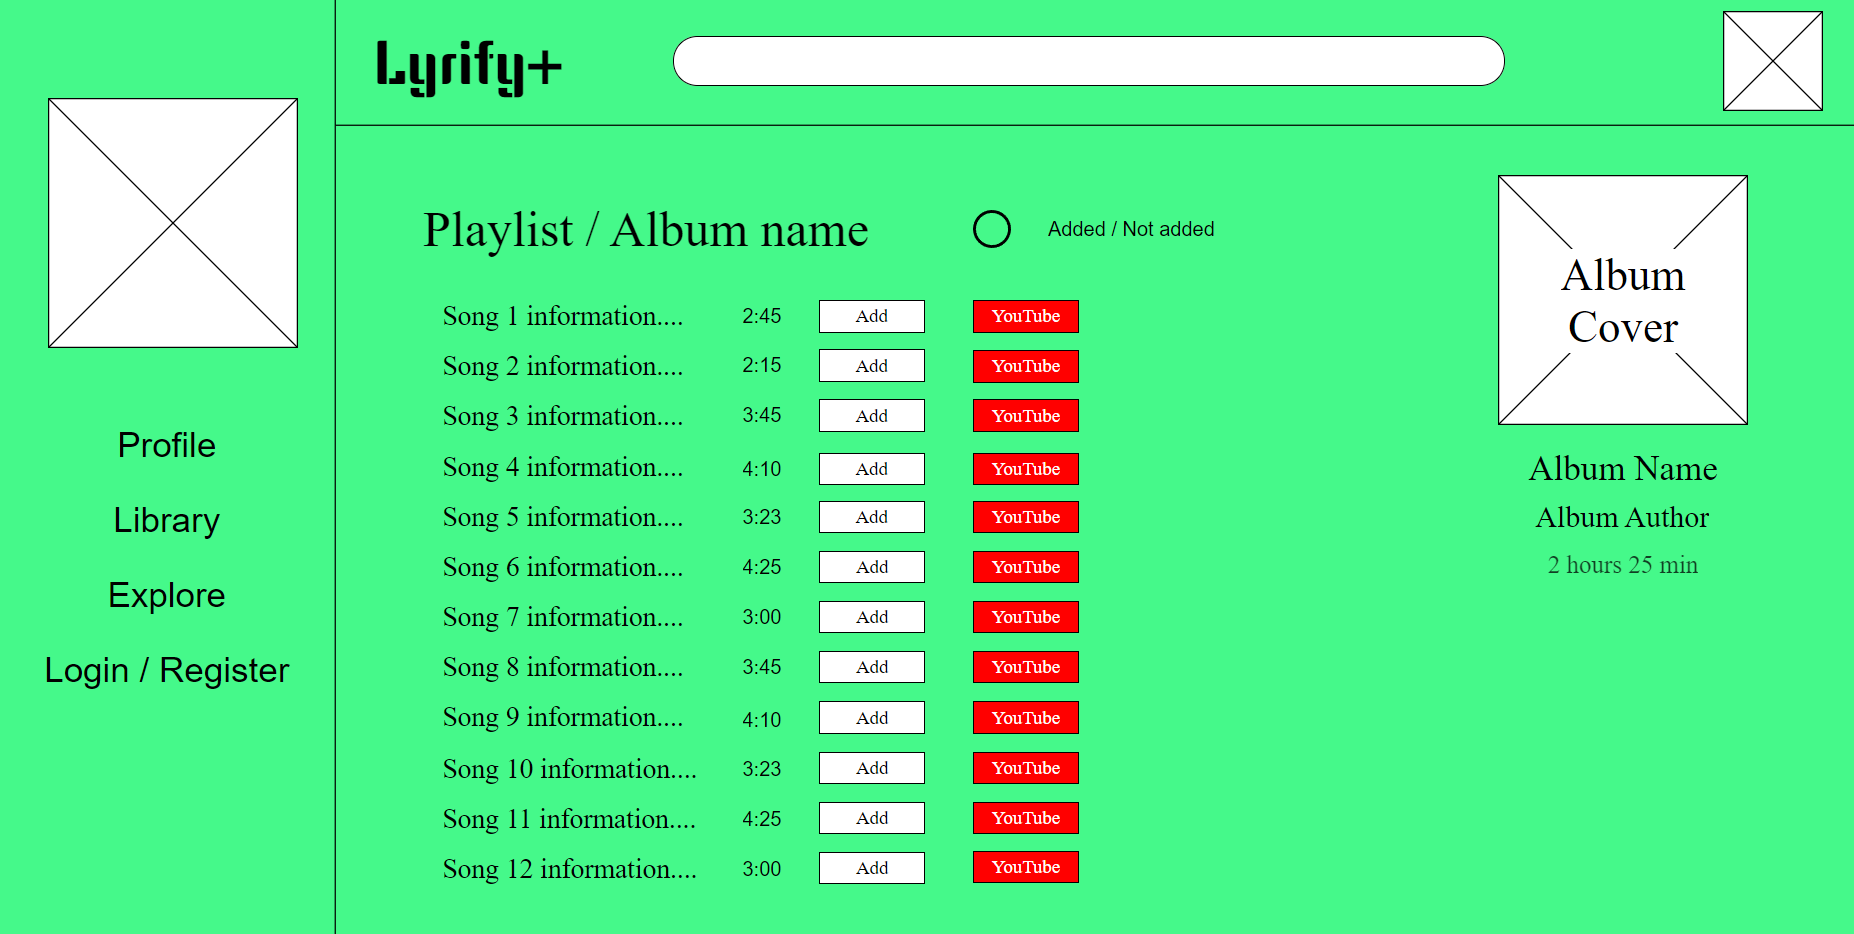
\includegraphics[width=0.9\textwidth]{sections/PLL/PlaylistPageMockup.png}
\caption{Playlist / Album page}
\end{figure}

For this page, the general design is maintained as always, regarding the side and top panels. Then, the info displayed in the page will depend on from where it is opened, because it will display info for playlists and albums.

As an album page, the album’s name will be displayed on top, next to it, an added button will appear selected in the case the album is added by the user or empty in case the user has not selected yet the album. On the right side, the album’s cover photo, name, author and complete duration will be displayed. And, in the center of the page, the list of songs belonging to the album will be displayed, showing the songs’ names, durations, add buttons and YouTube video buttons.

As a playlist page, the page will show the playlist’s name, and the list of songs with all the respective information regarding the songs.